\documentclass[sigconf]{acmart}
\usepackage{balance}

\settopmatter{printacmref=false}
\renewcommand\footnotetextcopyrightpermission[1]{}

% bold paragraph titles
\newcommand{\mypar}[1]{{\bf #1.}}

% Metadata
\title{Extending and Reproducing pSTL-Bench: oneDPL Backend Integration and Enhanced Reproducibility}

\author{Oleg Bilovus}
\affiliation{
  \institution{Department of Computer Science, University of Salerno}
  \city{Fisciano (SA)}
  \country{Italy}
}

\balance{}
\begin{document}

\begin{abstract}
  Describe in concise words what you do, why you do it (not necessarily
  in this order), and the main result.  The abstract has to be
  self-contained and readable for a person in the general area. You
  should write the abstract last.
\end{abstract}

\maketitle

\section{Introduction}\label{sec:intro}
Writing performance-portable and efficient parallel applications remains a
significant challenge due to the diversity of modern hardware architectures.
The emergence of parallel programming frameworks and, more recently, the
introduction of parallel algorithms in the \textit{C++17 Standard Template
  Library (STL)} aim to address this challenge by enabling developers to write
code that runs efficiently across CPUs and GPUs using a standardized interface.

\textit{pSTL-Bench}~\cite{pSTL-Bench} is a benchmark suite originally developed to
quantitatively evaluate the performance of individual parallel STL algorithms
across various compiler frameworks (such as GCC, Intel's icpx, NVIDIA HPC SDK)
and backends (including TBB, HPX, OpenMP, and CUDA). It provides a focused,
micro-benchmarking approach that avoids the complexities of full applications
and highlights the relative performance characteristics of different STL
implementations.

In this work, the main results and experiments from the original
pSTL-Bench paper are reproduced. Beyond reproduction, the project is
then extended by incorporating support for the \textit{oneAPI DPC++ Library
  (oneDPL)} backend, enabling the evaluation of Intel’s parallel STL
implementation based on the \textit{SYCL programming model} on both CPU and GPU
platforms

To further enhance the usability and reproducibility of the benchmark suite,
automation tools are introduced, including Ansible playbooks for environment
setup and benchmark execution, R scripts for performance analysis, and expanded
documentation for ease of deployment and adding new backends.

\mypar{Related Work} This work builds directly on pSTL-Bench.
While performance portability and parallelism have been widely studied in
the context of full applications and frameworks such as Kokkos~\cite{Kokkos}
and RAJA~\cite{RAJA}, no prior work has reproduced or extended pSTL-Bench,
nor added support for the oneDPL backend or focused on improving its reproducibility.

\section{Background: Whatever the Background is}\label{sec:background}

Give a short, self-contained summary of necessary background information. For
example, assume you present an implementation of sorting algorithms. You could
organize into sorting definition, algorithms considered, and asymptotic runtime
statements. The goal of the background section is to make the paper
self-contained for an audience as large as possible. As in every section you
start with a very brief overview of the section. Here it could be as follows:
In this section we formally define the sorting problem we consider and
introduce the algorithms we use including a cost analysis.

\mypar{Sorting}
Precisely define sorting problem you consider.

\mypar{Sorting algorithms}
Explain the algorithm you use including their costs.

As an aside, don't talk about "the complexity of the algorithm.'' It's
incorrect, problems have a complexity, not algorithms.

\section{Your Proposed Method}\label{sec:yourmethod}

Now comes the ``beef'' of the report, where you explain what you did. Again,
organize it in paragraphs with titles. As in every section you start with a
very brief overview of the section.

In this section, structure is very important so one can follow the technical
content.

Mention and cite any external resources that you used including libraries or
other code.

\section{Experimental Results}\label{sec:exp}

Here you evaluate your work using experiments. You start again with a very
short summary of the section. The typical structure follows.

\mypar{Experimental setup} Specify the platform (processor, frequency, maybe OS, maybe cache sizes)
as well as the compiler, version, and flags used. If your work is about performance,
I strongly recommend that you play with optimization flags and consider also icc for additional potential speedup.

Then explain what kind of benchmarks you ran. The idea is to give enough
information so the experiments are reproducible by somebody else on his or her
code. For sorting you would talk about the input sizes. For a tool that
performs NUMA optimization, you would specify the programs you ran.

\mypar{Results}
Next divide the experiments into classes, one paragraph for each. In each class of experiments you typically pursue one questions that then is answered by a suitable plot or plots. For example, first you may want to investigate the performance behavior with changing input size, then how your code compares to external benchmarks.

  {\bf Comments:}
\begin{itemize}
  \item Create very readable, attractive plots (do 1 column, not 2 column plots for
        this report) with readable font size. However, the font size should also not be
        too large; typically it is smaller than the text font size. An example is in
        Fig. (of course you can have a different style).
  \item Every plot answers a question. You state this question and extract the answer
        from the plot in its discussion.
  \item Every plot should be referenced and discussed.
\end{itemize}

\begin{figure}\centering
  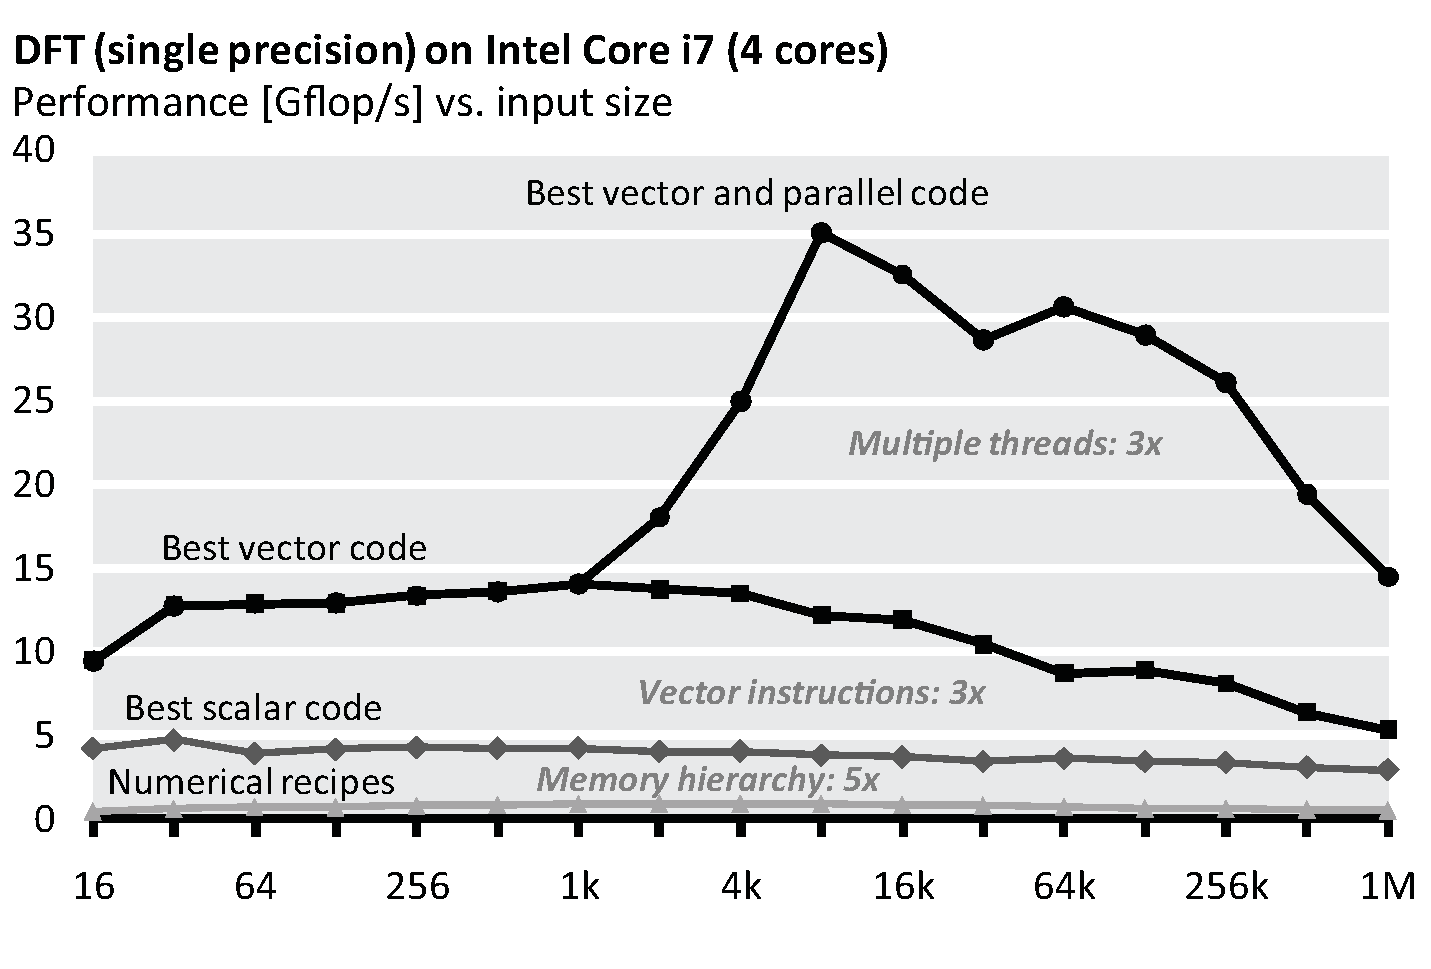
\includegraphics[scale=0.33]{example-plot}
  \caption{Performance of four single precision implementations of the
    discrete Fourier transform. The operations count is roughly the
    same. The labels in this plot are maybe a little bit too small.\label{fftperf}}
  \Description{A line plot comparing the performance of four single precision discrete Fourier transform implementations, showing similar operation counts and varying label sizes.}
\end{figure}

\section{Conclusions}

Here you need to summarize what you did and why this is important. {\em Do not
    take the abstract} and put it in the past tense. Remember, now the reader has
(hopefully) read the report, so it is a very different situation from the
abstract. Try to highlight important results and say the things you really want
to get across such as high-level statements (e.g., we believe that .... is the
right approach to .... Even though we only considered x, the .... technique
should be applicable ....) You can also formulate next steps if you want. Be
brief. After the conclusions there are only the references.

\section{Further comments}

Here we provide some further tips.

\mypar{Further general guidelines}

\begin{itemize}
  \item For short papers, to save space, I use paragraph titles instead of subsections,
        as shown in the introduction.

  \item It is generally a good idea to break sections into such smaller units for
        readability and since it helps you to (visually) structure the story.

  \item The above section titles should be adapted to more precisely reflect what you
        do.

  \item Each section should be started with a very short summary of what the reader can
        expect in this section. Nothing more awkward as when the story starts and one
        does not know what the direction is or the goal.

  \item Make sure you define every acronym you use, no matter how convinced you are the
        reader knows it.

  \item Always spell-check before you submit (to us in this case).

  \item Be picky. When writing a paper you should always strive for very high quality.
        Many people may read it and the quality makes a big difference. In this class,
        the quality is part of the grade.

  \item Books helping you to write better:.

  \item Conversion to pdf (latex users only):

        dvips -o conference.ps -t letter -Ppdf -G0 conference.dvi

        and then

        ps2pdf conference.ps
\end{itemize}

\mypar{Graphics} For plots that are not images {\em never} generate the bitmap formats
jpeg, gif, bmp, tif. Use eps, which means encapsulate postscript. It is
scalable since it is a vector graphic description of your graph. E.g.,
from Matlab, you can export to eps.

The format pdf is also fine for plots (you need pdflatex then), but only if the
plot was never before in the format jpeg, gif, bmp, tif.

\balance{}
\bibliographystyle{ACM-Reference-Format}
\begin{thebibliography}{1}

  \bibitem{pSTL-Bench}
  R. Laso, D. Krupitza, and S. Hunold, ``Exploring Scalability in C++ Parallel STL Implementations'' in \textit{Proceedings of the 53rd International Conference on Parallel Processing (ICPP '24)},
  Association for Computing Machinery, New York, NY, USA, 2024, pp. 284--293.
  \url{https://doi.org/10.1145/3673038.3673065}

  \bibitem{Kokkos}
  H. C. Edwards and C. R. Trott, ``Kokkos: Enabling Performance Portability Across Manycore Architectures'' \textit{2013 Extreme Scaling Workshop (xsw 2013)},
  Boulder, CO, USA, 2013, pp. 18-24.
  \url{https://doi.org/10.1109/XSW.2013.7}

  \bibitem{RAJA}
  D. A. Beckingsale et al., ``RAJA: Portable Performance for Large-Scale Scientific Applications'' \textit{2019 IEEE/ACM International Workshop on Performance, Portability and Productivity in HPC (P3HPC)},
  Denver, CO, USA, 2019, pp. 71-81.
  \url{https://doi.org/10.1109/P3HPC49587.2019.00012}

\end{thebibliography}

\end{document}

